\documentclass[
  bibliography=totoc,     % Literatur im Inhaltsverzeichnis
  captions=tableheading,  % Tabellenüberschriften
  titlepage=firstiscover, % Titelseite ist Deckblatt
]{scrartcl}

% Paket float verbessern
\usepackage{scrhack}

% Warnung, falls nochmal kompiliert werden muss
\usepackage[aux]{rerunfilecheck}

% unverzichtbare Mathe-Befehle
\usepackage{amsmath}
% viele Mathe-Symbole
\usepackage{amssymb}
% Erweiterungen für amsmath
\usepackage{mathtools}

% Fonteinstellungen
\usepackage{fontspec}
% Latin Modern Fonts werden automatisch geladen
% Alternativ zum Beispiel:
%\setromanfont{Libertinus Serif}
%\setsansfont{Libertinus Sans}
%\setmonofont{Libertinus Mono}

% Wenn man andere Schriftarten gesetzt hat,
% sollte man das Seiten-Layout neu berechnen lassen
\recalctypearea{}

% deutsche Spracheinstellungen
\usepackage{polyglossia}
\setmainlanguage{german}


\usepackage[
  math-style=ISO,    % ┐
  bold-style=ISO,    % │
  sans-style=italic, % │ ISO-Standard folgen
  nabla=upright,     % │
  partial=upright,   % ┘
  warnings-off={           % ┐
    mathtools-colon,       % │ unnötige Warnungen ausschalten
    mathtools-overbracket, % │
  },                       % ┘
]{unicode-math}

% traditionelle Fonts für Mathematik
\setmathfont{Latin Modern Math}
% Alternativ zum Beispiel:
%\setmathfont{Libertinus Math}

\setmathfont{XITS Math}[range={scr, bfscr}]
\setmathfont{XITS Math}[range={cal, bfcal}, StylisticSet=1]

% Zahlen und Einheiten
\usepackage[
  locale=DE,                   % deutsche Einstellungen
  separate-uncertainty=true,   % immer Fehler mit \pm
  per-mode=symbol-or-fraction, % / in inline math, fraction in display math
]{siunitx}

% chemische Formeln
\usepackage[
  version=4,
  math-greek=default, % ┐ mit unicode-math zusammenarbeiten
  text-greek=default, % ┘
]{mhchem}

% richtige Anführungszeichen
\usepackage[autostyle]{csquotes}

% schöne Brüche im Text
\usepackage{xfrac}

% Standardplatzierung für Floats einstellen
\usepackage{float}
\floatplacement{figure}{htbp}
\floatplacement{table}{htbp}

% Floats innerhalb einer Section halten
\usepackage[
  section, % Floats innerhalb der Section halten
  below,   % unterhalb der Section aber auf der selben Seite ist ok
]{placeins}

% Seite drehen für breite Tabellen: landscape Umgebung
\usepackage{pdflscape}

% Captions schöner machen.
\usepackage[
  labelfont=bf,        % Tabelle x: Abbildung y: ist jetzt fett
  font=small,          % Schrift etwas kleiner als Dokument
  width=0.9\textwidth, % maximale Breite einer Caption schmaler
]{caption}
% subfigure, subtable, subref
\usepackage{subcaption}

% Grafiken können eingebunden werden
\usepackage{graphicx}
% größere Variation von Dateinamen möglich
\usepackage{grffile}

% schöne Tabellen
\usepackage{booktabs}

% Verbesserungen am Schriftbild
\usepackage{microtype}

% Literaturverzeichnis
\usepackage[
  backend=biber,
]{biblatex}
% Quellendatenbank
\addbibresource{lit.bib}
\addbibresource{programme.bib}

% Hyperlinks im Dokument
\usepackage[
  unicode,        % Unicode in PDF-Attributen erlauben
  pdfusetitle,    % Titel, Autoren und Datum als PDF-Attribute
  pdfcreator={},  % ┐ PDF-Attribute säubern
  pdfproducer={}, % ┘
]{hyperref}
% erweiterte Bookmarks im PDF
\usepackage{bookmark}

% Trennung von Wörtern mit Strichen
\usepackage[shortcuts]{extdash}

\author{%
  Jan Philipp Jäkel\\%
  \href{mailto:jan.jaekel@tu-dortmund.de}{jan.jaekel@tu-dortmund.de}%
  \texorpdfstring{\and}{,}%
  Piet Hoffmann\\%
  \href{mailto:piet.hoffmann@tu-dortmund.de}{piet.hoffmann@tu-dortmund.de}%
}
\publishers{TU Dortmund – Fakultät Physik}


\subject{v107}
\title{Das Kugelfallviskosimeter nach Höppler}

\date{
  \begin{align}
    \text{Durchführung: } & \text{12.12.2017} & \hspace{3em} & \text{Abgabe: 19.12.2017} \notag
%\\  \text{Korrektur: } & \text{22.11.2017} & \hspace {3em} & \notag 
  \end{align}
}

%\date{%
%  Durchführung: DATUM
%  \hspace{3em}
%  Abgabe: DATUM
%}

\begin{document}

\maketitle
\thispagestyle{empty}
\tableofcontents
\newpage

\section{Zielsetzung}
Ziel dieses Versuchs ist es die Temperaturabhängigkeit der dynamischen Viskosität von destilliertem Wasser, mittels Kugelfall-Viskosimeter, zu bestimmen.
\section{Theorie}
\label{sec:Theorie}
Auf einen Körper wirkt eine Reibungskraft, welche von der Berührungsfläche $A$ und der Geschwindigkeit abhängt, sofern sich dieser durch eine Flüssigkeit bewegt.
Die Flüssigkeit selbst wird durch eine Materialkonstante und die dynamische Viskosität $\eta$ beschrieben.
Diese kann unter Verwendung eines Kugelfall-Viskosimeter bestimmt werden.
Viskosität bezeichnet das Maß an "fließfhigkeit" einer Flüßigkeit.
Ist die Viskosität größer, dann ist die Bindung der Teilchen stärker und somit auch die beweglichkeit geringer.
Hierbei fällt eine Kugel mit Radius $r$ in einer Flüssigkeit, sodass keine Wirbel entstehen.
Die Strömung ist dann laminar. Umgekehrt würde die Strömung als turbulent bezeichnet werden, wenn Wirbel in der Flüssigkeit entstehen würden.
Dann kann die Stokessche Reibung durch
\begin{equation}
  F_R = 6 \pi \eta \upsilon r
\end{equation}
angeben werden, wobei $\upsilon$ die Fallgeschwindigkeit darstellt.
Neben der Reibungskraft wirken auf die Kugel die Schwerkraft $F_g$ und der Auftrieb $F_A$.
Auftrieb und Schwerkraft sind entgegengerichtet.
\subsection{Aufbau}
Um die Viskosität zu betimmen wird hier das Kugelfall-Viskosimeter nach Höppler verwendet.
Die Abbildung \ref{fig:aufbau} zeigt dieses.
\begin{figure}
  \centering
  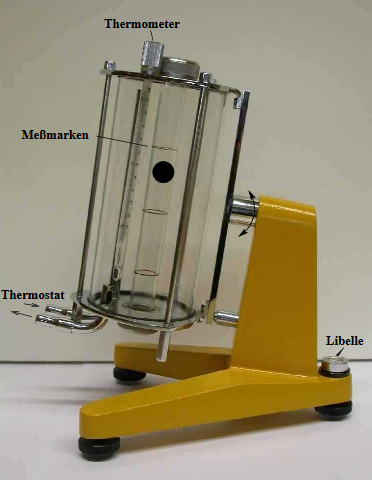
\includegraphics{content/Aufbau.png}
  \caption{Kugelfall-Viskosimeter nach Höppler\cite{v107}}
  \label{fig:aufbau}
\end{figure}
Bei diesem wird eine Kugel in einem Rohr fallengelassen, welches einen geringfügig größeren Durchmesser als die Kugel aufweist.
Das Rohr ist dabei mit einer viskosen Flüssigkeit gefüllt.
Um zu vermeiden, dass die Kugel unkontrolliert gegen die Rohrwand stößt ist das Fallrohr leicht geneigt, sodass die Kugel die Rohrwand hinabgleitet.
Bei konstanter Temperatur lässt sich die Viskosität der Flüssigkeit durch
\begin{equation}
  \upeta = K (\rho_K -\rho_\text{Fl}) \cdot t
\end{equation}
 berechnen.
Hier ist $\rho_K$ die Dichte der Kugel, $\rho_\text{Fl}$ die Dichte der Flüssigkeit, $t$ die Fallzeit der Kugel und $K$ eine Apparaturkonstante, welche sowohl die Fallhöhe als auch die Kugelgeometrie enthält.
Die Viskosität vieler Flüssigkeiten ist stark Temperaturabhängig.
Andradesches Gleichung beschreibt die Viskosität bei variabler Temperatur:
\begin{equation}
  \label{eq:and}
  \upeta (T)= A \exp(\frac{B}{T})
\end{equation}
A und B sind dabei Konstanten.
Die Temperatur der viskosen Flüssigkeit lässt sich über ein Wasserbad regulieren, welches durch zwei Zylinder realisiert wird.
Nachdem die Kugel am Ende des Fallrohrs angekommen ist kann das Viskosimeter um $180$ Grad rotiert werden.
\subsection{Die Reynoldsche Zahl}
Die Reynoldsche Zahl ist eine dimensionslose Kenngröße.
Sie findet Verwendung bei der Untersuchung ob eine Strömung turbulent oder laminar ist.
Überschreitet diese einen kirtischen Wert, so ist die Strömung turbulent.
Für Wasser liegt dieser Wert bei $R_e=2300$\cite{ström}.
Die Reynoldsche Zahl ist durch
\begin{equation}
  R_e = \frac{\rho \nu d}{\upeta}
\end{equation}
definiert.
Hierbei ist \rho die Dichte der Flüssigkeit, \nu die Strömungsgeschwindigkeit der Flüßigkeit gegenüber des Körpers und $d$ die Länge des Körpers.

\section{Durchführung}
\label{sec:Durchführung}

\section{Auswertung}
\label{sec:Auswertung}
\subsection{Bestimmung der Viskosität von destilliertem Wasser bei konstanter Temperatur}
Die Viskosität von destilliertem Wasser bei konstanter Temperatur lässt sich über die Gleichung\eqref{eq:dicht} berechnen.
Die Dichte der Kugel erhält man aus den gemessenen Werten für die Masse und den Durchmesser, welche in Tabelle aufgetragen sind.
\begin{table}[H]
  \caption{Ergebnisse der Messung.}
  \label{tab:kl_maße}
  \centering
  \sisetup{table-format=2.2}
  \begin{tabular}{cSSS}
    \toprule
    \midrule
    {$m/\si{\gram}$} & 4.45 & 4.44 & 4.46 \\
    {$D/\si{\milli\meter}$} & 15.59 & 15.60 & 15.59 \\
    \bottomrule
  \end{tabular}
\end{table}
\noindent Im Mittel erhält man dann für den Durchmesser und die Masse:
\begin{equation*}
  \bar{m}=\SI{4.45\pm 0.01}{\gram}
\end{equation*}
\begin{equation*}
  \bar{D}=\SI{15.59\pm 0.14 }{\milli\meter}
\end{equation*}
\noindent Die Ungenauigkeit errechnet sich hier über Streung des Mittelwertes:
 \begin{equation}
   \Delta \bar{x} =\sqrt{\frac{1}{N(N-1)}\sum_{i=1}^N(x_i-\bar{x})^2}
 \end{equation}
\begin{table}[H]
    \centering
    \caption{Fallzeiten der kleinen Kugel.}
    \label{tab:kl_fall}
    \begin{tabular}{S[table-format=2.2] S[table-format=2.2] }
        \toprule
        {$1.Messung/\si{\second}$} & {$2.Messung/\si{\second}$} \\
        \midrule
        12.22   & 12.29 \\
        12.22   & 12.07 \\
        12.16   & 12.18 \\
        12.19   & 12.07 \\
        12.22   & 12.13 \\
        \bottomrule
    \end{tabular}
\end{table}


\subsection{Bestimmung der Apparaturkonstante für die große Kugel}
\subsection{Berechnung der Reynoldschen Zahl}

\section{Diskussion}
Damit die Gleichungen, welche hier verwendet werden, gelten muss die Strömung im Fallrohr laminar sein.
Aus den berechneten Werten für Reynolds-Zahlen folgt, dass diese hier ein bis zwei Größenordungen von dem kritischen Wert entfernt sind.
Es lässt sich also mit größer Sicherheit davon ausgehen, dass die Strömung im Rohr laminar ist.
Da der Versuch in einem geschlossenen System stattfindet sind auch die systematischen Fehlerquellen gering und finden sich hauptsächlich in der Zeitmessung.


\printbibliography{}

\end{document}
